\documentclass[addpoints,12pt]{exam}
\usepackage{amsmath}
\usepackage{amsthm}
\usepackage{amsfonts}
\usepackage{systeme}
\usepackage{graphicx}
\usepackage{caption}
\usepackage{xfrac}
\usepackage{physics}
\usepackage{microtype}
\usepackage{eulervm}
%\usepackage[framemethod=tikz]{mdframed}
\usepackage{thmtools}
\usepackage{etoolbox}
%\usepackage{fouriernc}
\usepackage{mdframed}
\usepackage[overload]{empheq}
\usepackage{adjustbox}
\usepackage{enumitem}
\usepackage[explicit]{titlesec}
% adds in \varnothing for empty set
\usepackage{amssymb}
% adds in formated SI units
%\usepackage{siunitx}
\usepackage{pgfplots}
\usepackage{multirow}
\usepackage{array}

\pagestyle{headandfoot}
\runningfootrule
\firstpageheadrule
\runningheadrule

\newcommand{\class}{Math 0098}
\newcommand{\sem}{2211}
\newcommand{\due}{}
\newcommand{\sect}{11.1}
\newcommand{\topic}{More on Quadratics}

\firstpageheader{\class}{\sect - \topic}{}
\runningheader{\class}{\sect - \topic}{}
\firstpagefooter{\class}{}{Page \thepage\ of \numpages}
\runningfooter{\class}{}{Page \thepage\ of \numpages}

\newif\ifprintselected
\printselectedtrue
%\printselectedfalse

\newenvironment{select}
{\ifprintselected
	\printanswers
	\fi
}
{}

\theoremstyle{definition}
\newtheorem{theorem}{Theorem}
%\newtheorem{example}{Example}[subsection]
%\newtheorem{definition}{Definition}
%\newmdtheoremenv{definition}{Definition}[subsection]
%\newmdtheoremenv{example}{Example}[subsection]
\AtBeginEnvironment{defn}{\begin{minipage}{\textwidth}}
\AtEndEnvironment{defn}{\end{minipage}}
%\AtBeginEnvironment{example}{\begin{minipage}{\textwidth}}
%\AtEndEnvironment{example}{\end{minipage}}
\newcommand{\iu}{{i\mkern1mu}}

\setlength{\gridsize}{5mm}
\setlength{\gridlinewidth}{0.1pt}

\printanswers
\DeclareMathSizes{12}{12}{12}{12}

%%%%%%%%%%%%%%%%%%%%%%%%
% Create bars around subsubsection
%%%%%%%%%%%%%%%%%%%%%%%%

\titleformat{\subsubsection}
   {\large\bfseries}% format
   {}% label
   {0pt}% sep
   {\titlerule \vspace{.1in} #1}% before code
      [{\titlerule[0.4pt]\vspace{.1in}}]% after code
\titlespacing{\subsubsection}
   {0pt}% left
   {0pt}% before sep
   {\baselineskip}% after sep
   
%%%%%%%%%%%%%%%%%%%%%%%
% Create line break after definition label
%%%%%%%%%%%%%%%%%%%%%%%   
\newtheoremstyle{break}
  {\topsep}{\topsep}%
  {}{}%\itshape
  {\bfseries}{}%
  {\newline}{}%
\theoremstyle{break}
\newmdtheoremenv{definition}{Definition}[subsection]
\theoremstyle{break}
\newtheorem{example}{Example}[subsection]

%%%%%%%%%%%%%%%%%%%%%%
% start document
% set section, subsection (use n-1 for sub)
%%%%%%%%%%%%%%%%%%%%%%


\begin{document}
\setcounter{section}{11}
\setcounter{subsection}{0}

\subsection{More on Quadratics}
We've worked with quadratics frequently throughout this class -- factoring quadratics, identifying roots, evaluating, etc. Chapter 11 delves deeper into the properties of quadratic functions.
\vspace{.2in}
\subsubsection*{The Square Root Property}

Consider the simple quadratic equation $x^2-4=0$. We could solve this by difference of squares.
\begin{eqnarray*}
x^2 - 4 &=& x^2 - 2^2\\
&=& (x-2)(x+2)
\end{eqnarray*}

This method yields solutions of $x=2$ and $x=-2$. However, you might notice that we could solve this in a different manner as well. Notice that there is no \emph{linear term} -- there is no term that has just an $x$. Because of this, we can use the square root property to solve.

\begin{eqnarray*}
x^2 - 4 &=& 0\\
x^2 &=& 4\\
x &=& \pm\sqrt{4}\\
x &=& \pm 2
\end{eqnarray*}

\vspace{.2in}

\begin{mdframed}
\textbf{The Square Root Property}\mbox{}\\
Let $u$ be an algebraic expression and $d$ be a non-zero real number. If $u^2 = d$, then $u=\pm\sqrt{d}$. Mathematically, \[u^2=d \implies u=\pm\sqrt{d}\]
\end{mdframed}

\vspace{.2in}

\begin{example}
Solve the following using the square root property.
\[ 4x^2 = 28\]
\vspace{1.5in}
\end{example}

\begin{example}
Solve the following using the square root property.
\[ 3x^2-11=0\]
\vspace{1.5in}
\end{example}

\begin{example}
Solve the following using the square root property.
\[ 4x^2 +9 = 0\]
\vspace{1.5in}
\end{example}

\begin{example}
Solve the following using the square root property.
\[ (x-3)^2 = 10\]
\vspace{1.5in}
\end{example}

\newpage

\subsubsection*{Completing the Square}

We have introduced several methods of factoring quadratics so far. Now we introduce another. This method, completing the square, is a method that shows up frequently in various places. We will see it again later in this chapter when we find vertex form of a quadratic. It seems as if everyone teaches this method in a slightly different manner. There is no single correct method for applying this; instead, it can be setup and started differently depending on the context and application. If you were taught this method slightly differently, then please use whatever is more comfortable to you.

\vspace{.2in}

\begin{mdframed}
\textbf{Completing the Square}\mbox{}\\
Let $x^2 + bx + c = 0$ be a quadratic equation. By adding $\left(\sfrac{b}{2}\right)^2$ to both sides, we are able to rewrite the quadratic in a more factored form as $(x+\sfrac{b}{2})^2 +a = \left(\sfrac{b}{2}\right)^2$. We can then use the square root property to solve for $x$. Note that $a=1$ for this method to work. If $a\neq 1$, then we must divide through by $a$ before applying the method.
\end{mdframed}

\vspace{.2in}

\begin{example}
Solve the following by using the completing the square method.
\[ x^2 + 4x - 1 = 0\]

\vspace{2in}
\end{example}

\newpage
\begin{example}
Solve the following by using the completing the square method.
\[ 2x^2 + 3x - 4 = 0\]
\vspace{3in}
\end{example}

\begin{example}
Solve the following by using the completing the square method.
\[ 3x^2 - 9x + 8 = 0\]
\end{example}

\newpage

\subsubsection*{The Distance Formula}
Back in Algebra 1, we discussed plotting points on an $xy$-plane, finding the equations of lines that contain specific points, finding the slope of the line between points and many other such concepts. Using the tools that we now have at our disposal (namely quadratics), we can add two other concepts to our list -- distance between points and the midpoint (the point directly between two others).

\vspace{.2in}

The distance formula is derived from the Pythagorean theorem, $a^2 + b^2 = c^2$. If we have two points, $P_1(x_1,y_1)$ and $P_2(x_2,y_2)$ and want to find the distance between them, we start by making an imaginary right triangle (think way back to everyone's favorite class - geometry). We can find the length of the two legs of the triangle by subtracting the $x$ values for one leg (the \emph{run}) and subtracting the $y$ values for the other (the \emph{rise}). These two legs represent $a$ and $b$ in the Pythagorean theorem. The hypoteneuse, $c$, is the distance between the two points and is the quantity we need to find.

\vspace{.2in}
\begin{figure}[h]
\centering
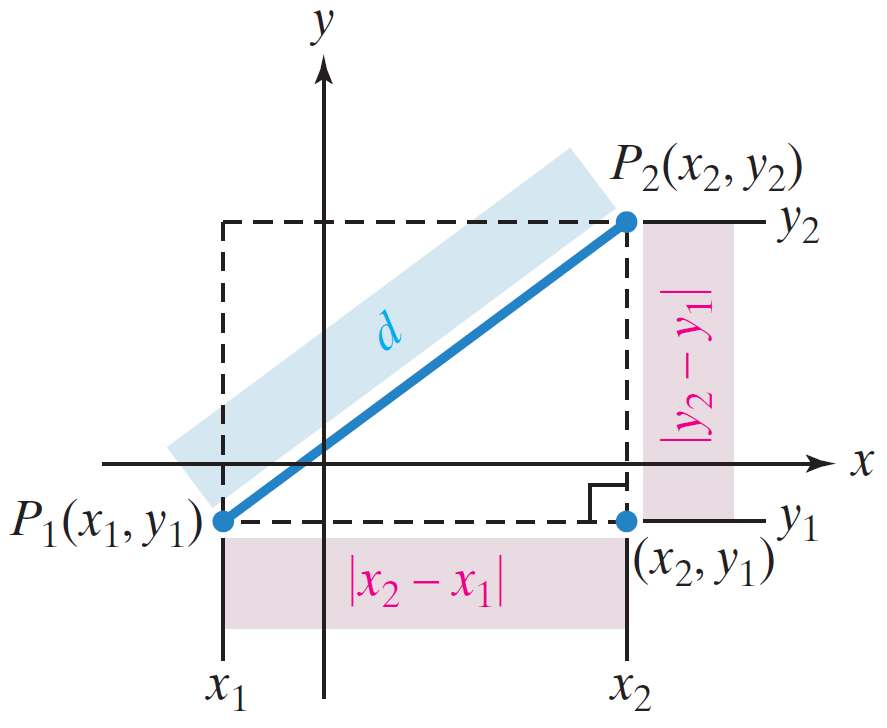
\includegraphics[scale=.25]{images/11_1_pyth_distance}
\end{figure}

By subtracting the two $x$ values, we get $a=\abs{x_1-x_2}$ -- why the absolute value? Since this represents a distance, it should be positive and the distance should be the same whether I start measuring from $x_1$ or from $x_2$. Similarly, subtracting the $y$ values we get $b=\abs{y_1-y_2}$. For ease of reading, replace $c$ with $d$ and now we can derive the distance formula.

\begin{eqnarray*}
c^2 &=& a^2 + b^2\\
d^2 &=& (x_1-x_2)^2 + (y_1-y_2)^2\\
d &=& \pm\sqrt{(x_1-x_2)^2 + (y_1-y_2)^2}\\
d &=& \sqrt{(x_1-x_2)^2 + (y_1-y_2)^2}
\end{eqnarray*}

\newpage

\begin{example}
Find the distance between the points $(-1,-3)$ and $(2,3)$. Give the distance as a reduced radical and as a decimal rounded to two places.
\vspace{2in}
\end{example}

\subsubsection*{The Midpoint Formula}
The midpoint of two points is the, well, \emph{point} in the \emph{mid}dle of two others. It's found by averaging the $x$ values and the $y$ values. The formula for the midpoint is \[mp = \left(\dfrac{x_1+x_2}{2},\dfrac{y_1+y_2}{2}\right)\]

\vspace{.2in}

\begin{example}
Find the midpoint of the points $(1,2)$ and $(7,-3)$.
\vspace{1in}
\end{example}


\end{document}